% Message sequence of one epoch of counterparty co-commitment (compiled to F4_protocol.pdf; included by main.tex)
\documentclass[tikz,border=3pt]{standalone}
\usepackage{amsmath,amssymb}
\usetikzlibrary{arrows.meta,calc}
\newcommand{\Sk}{\mathsf{Sk}}
\begin{document}
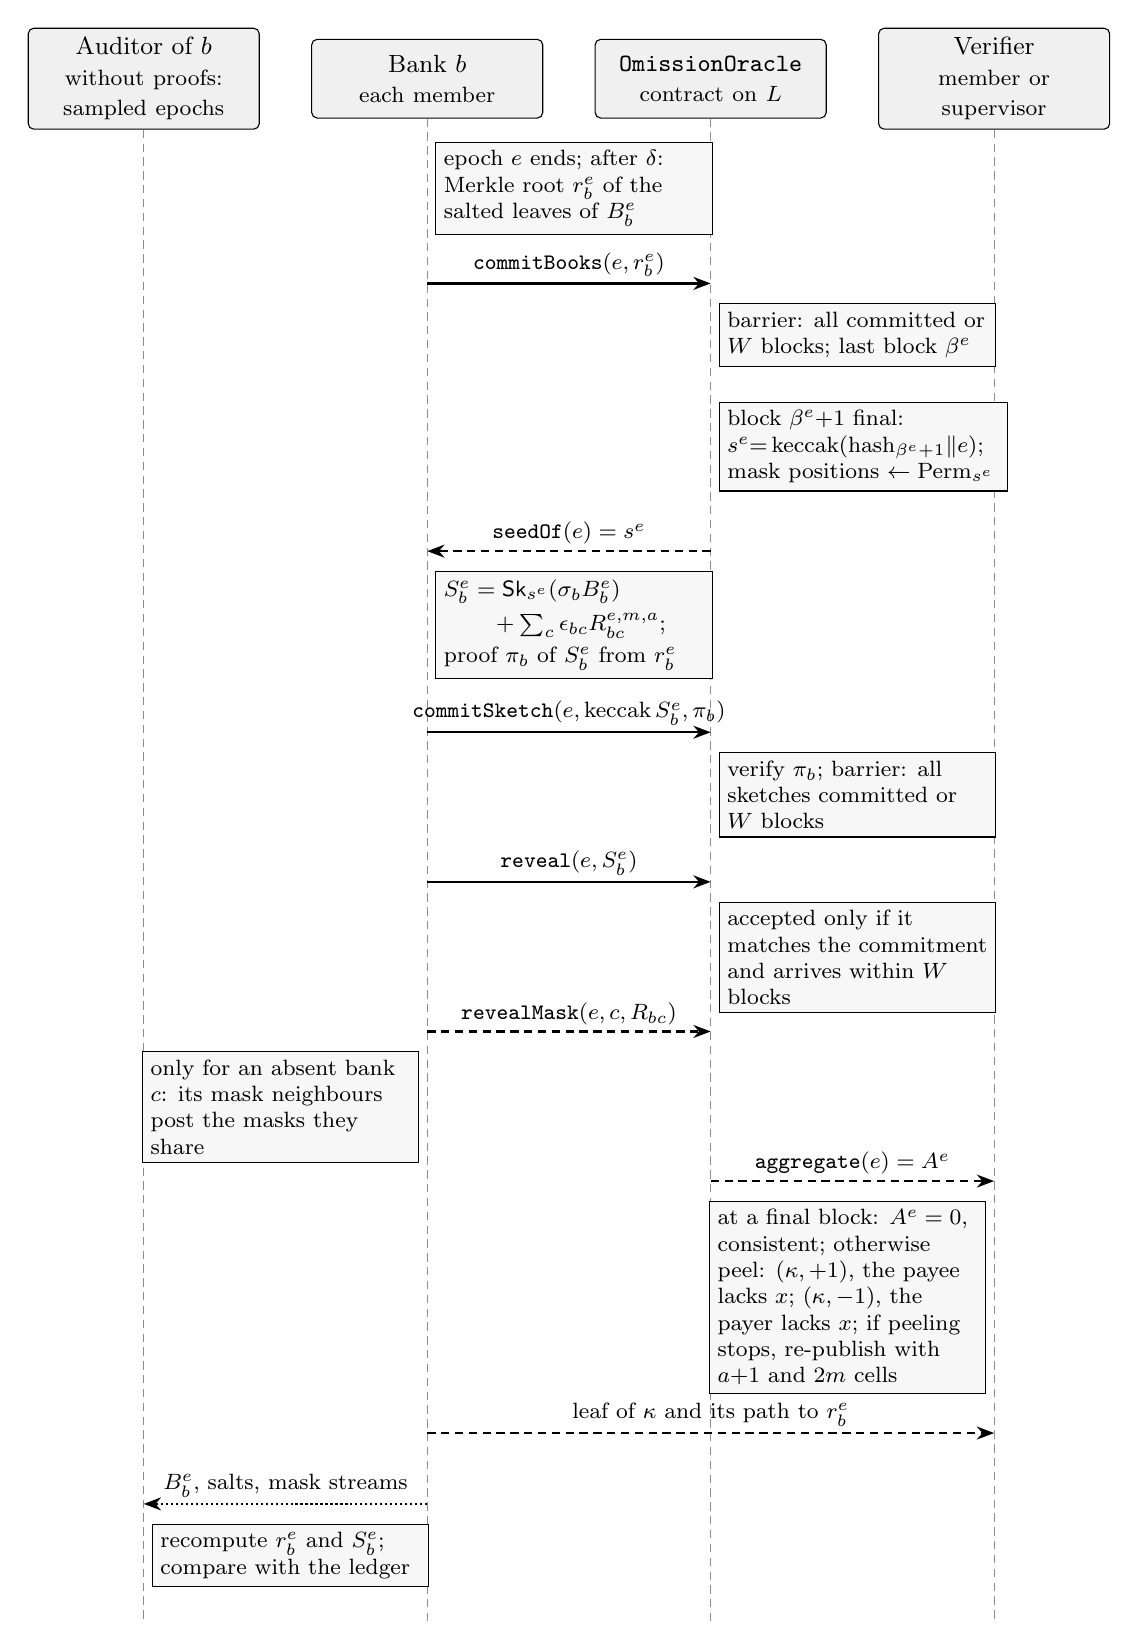
\begin{tikzpicture}[
  font=\small,
  head/.style={draw, rounded corners=2pt, fill=black!6, align=center, minimum height=1cm, text width=2.7cm},
  life/.style={densely dashed, black!45},
  note/.style={draw, fill=black!3, align=flush left, font=\footnotesize, inner sep=3pt, text width=#1},
  note/.default=3.3cm,
  msg/.style={-{Stealth[length=2.2mm]}, thick},
  rd/.style={-{Stealth[length=2.2mm]}, thick, densely dashed},
  lbl/.style={font=\footnotesize, above, inner sep=2pt},
]
\def\xa{0}\def\xb{3.6}\def\xc{7.2}\def\xd{10.8}\def\bot{-19.6}
\node[head] (A) at (\xa,0) {Auditor of $b$\\\footnotesize without proofs: sampled epochs};
\node[head] (B) at (\xb,0) {Bank $b$\\\footnotesize each member};
\node[head] (C) at (\xc,0) {\texttt{OmissionOracle}\\\footnotesize contract on $L$};
\node[head] (D) at (\xd,0) {Verifier\\\footnotesize member or supervisor};
\foreach \x/\n in {\xa/A,\xb/B,\xc/C,\xd/D} \draw[life] (\n.south) -- (\x,\bot);

% (1) books
\node[note, anchor=north west] at (\xb+0.1,-0.8) {epoch $e$ ends; after $\delta$: Merkle root $r^e_b$ of the salted leaves of $B^e_b$};
\draw[msg] (\xb,-2.6) -- node[lbl]{\texttt{commitBooks}$(e, r^e_b)$} (\xc,-2.6);

% (2) seed
\node[note, anchor=north west] at (\xc+0.1,-2.85) {barrier: all committed or $W$ blocks; last block $\beta^e$};
\node[note=3.45cm, anchor=north west] at (\xc+0.1,-4.1) {block $\beta^e{+}1$ final:\\$s^e{=}\,\mathrm{keccak}(\mathrm{hash}_{\beta^e+1}\|e)$;\\mask positions $\gets\mathrm{Perm}_{s^e}$};
\draw[rd] (\xc,-6.0) -- node[lbl]{\texttt{seedOf}$(e)=s^e$} (\xb,-6.0);

% (3) sketch commitment with its binding proof
\node[note, anchor=north west] at (\xb+0.1,-6.25) {$S^e_b=\Sk_{s^e}(\sigma_b B^e_b)$\\[3pt]$\qquad{}+\textstyle\sum_c \epsilon_{bc} R^{e,m,a}_{bc}$;\\[2pt]proof $\pi_b$ of $S^e_b$ from $r^e_b$};
\draw[msg] (\xb,-8.3) -- node[lbl]{\texttt{commitSketch}$(e,\mathrm{keccak}\,S^e_b,\pi_b)$} (\xc,-8.3);
\node[note, anchor=north west] at (\xc+0.1,-8.55) {verify $\pi_b$; barrier: all sketches committed or $W$ blocks};

% (4) reveal, dropouts
\draw[msg] (\xb,-10.2) -- node[lbl]{\texttt{reveal}$(e, S^e_b)$} (\xc,-10.2);
\node[note, anchor=north west] at (\xc+0.1,-10.45) {accepted only if it matches the commitment and arrives within $W$ blocks};
\draw[rd] (\xb,-12.1) -- node[lbl]{\texttt{revealMask}$(e,c,R_{bc})$} (\xc,-12.1);
\node[note, anchor=north east] at (\xb-0.1,-12.35) {only for an absent bank $c$: its mask neighbours post the masks they share};

% decoding and the follow-up
\draw[rd] (\xc,-14.0) -- node[lbl]{\texttt{aggregate}$(e)=A^e$} (\xd,-14.0);
\node[note, anchor=north east] at (\xd-0.1,-14.25) {at a final block: $A^e=0$, consistent; otherwise peel: $(\kappa,{+}1)$, the payee lacks $x$; $(\kappa,{-}1)$, the payer lacks $x$; if peeling stops, re-publish with $a{+}1$ and $2m$ cells};
\draw[rd] (\xb,-17.2) -- node[lbl]{leaf of $\kappa$ and its path to $r^e_b$} (\xd,-17.2);

% audit, where proofs are not used
\draw[msg, densely dotted] (\xb,-18.1) -- node[lbl]{$B^e_b$, salts, mask streams} (\xa,-18.1);
\node[note, anchor=north west] at (\xa+0.1,-18.35) {recompute $r^e_b$ and $S^e_b$; compare with the ledger};
\end{tikzpicture}
\end{document}
